\section{Google API configuratie}
\label{sec:google-api}
Dit hoofdstuk bevat een gedetailleerd stappenplan voor het configureren van een Google API. De Python demofunctie maakt gebruik van de Google API voor het wegschrijven van data naar Google spreadsheets.

\begin{figure}[h]
    \begin{subfigure}{0.5\textwidth}
        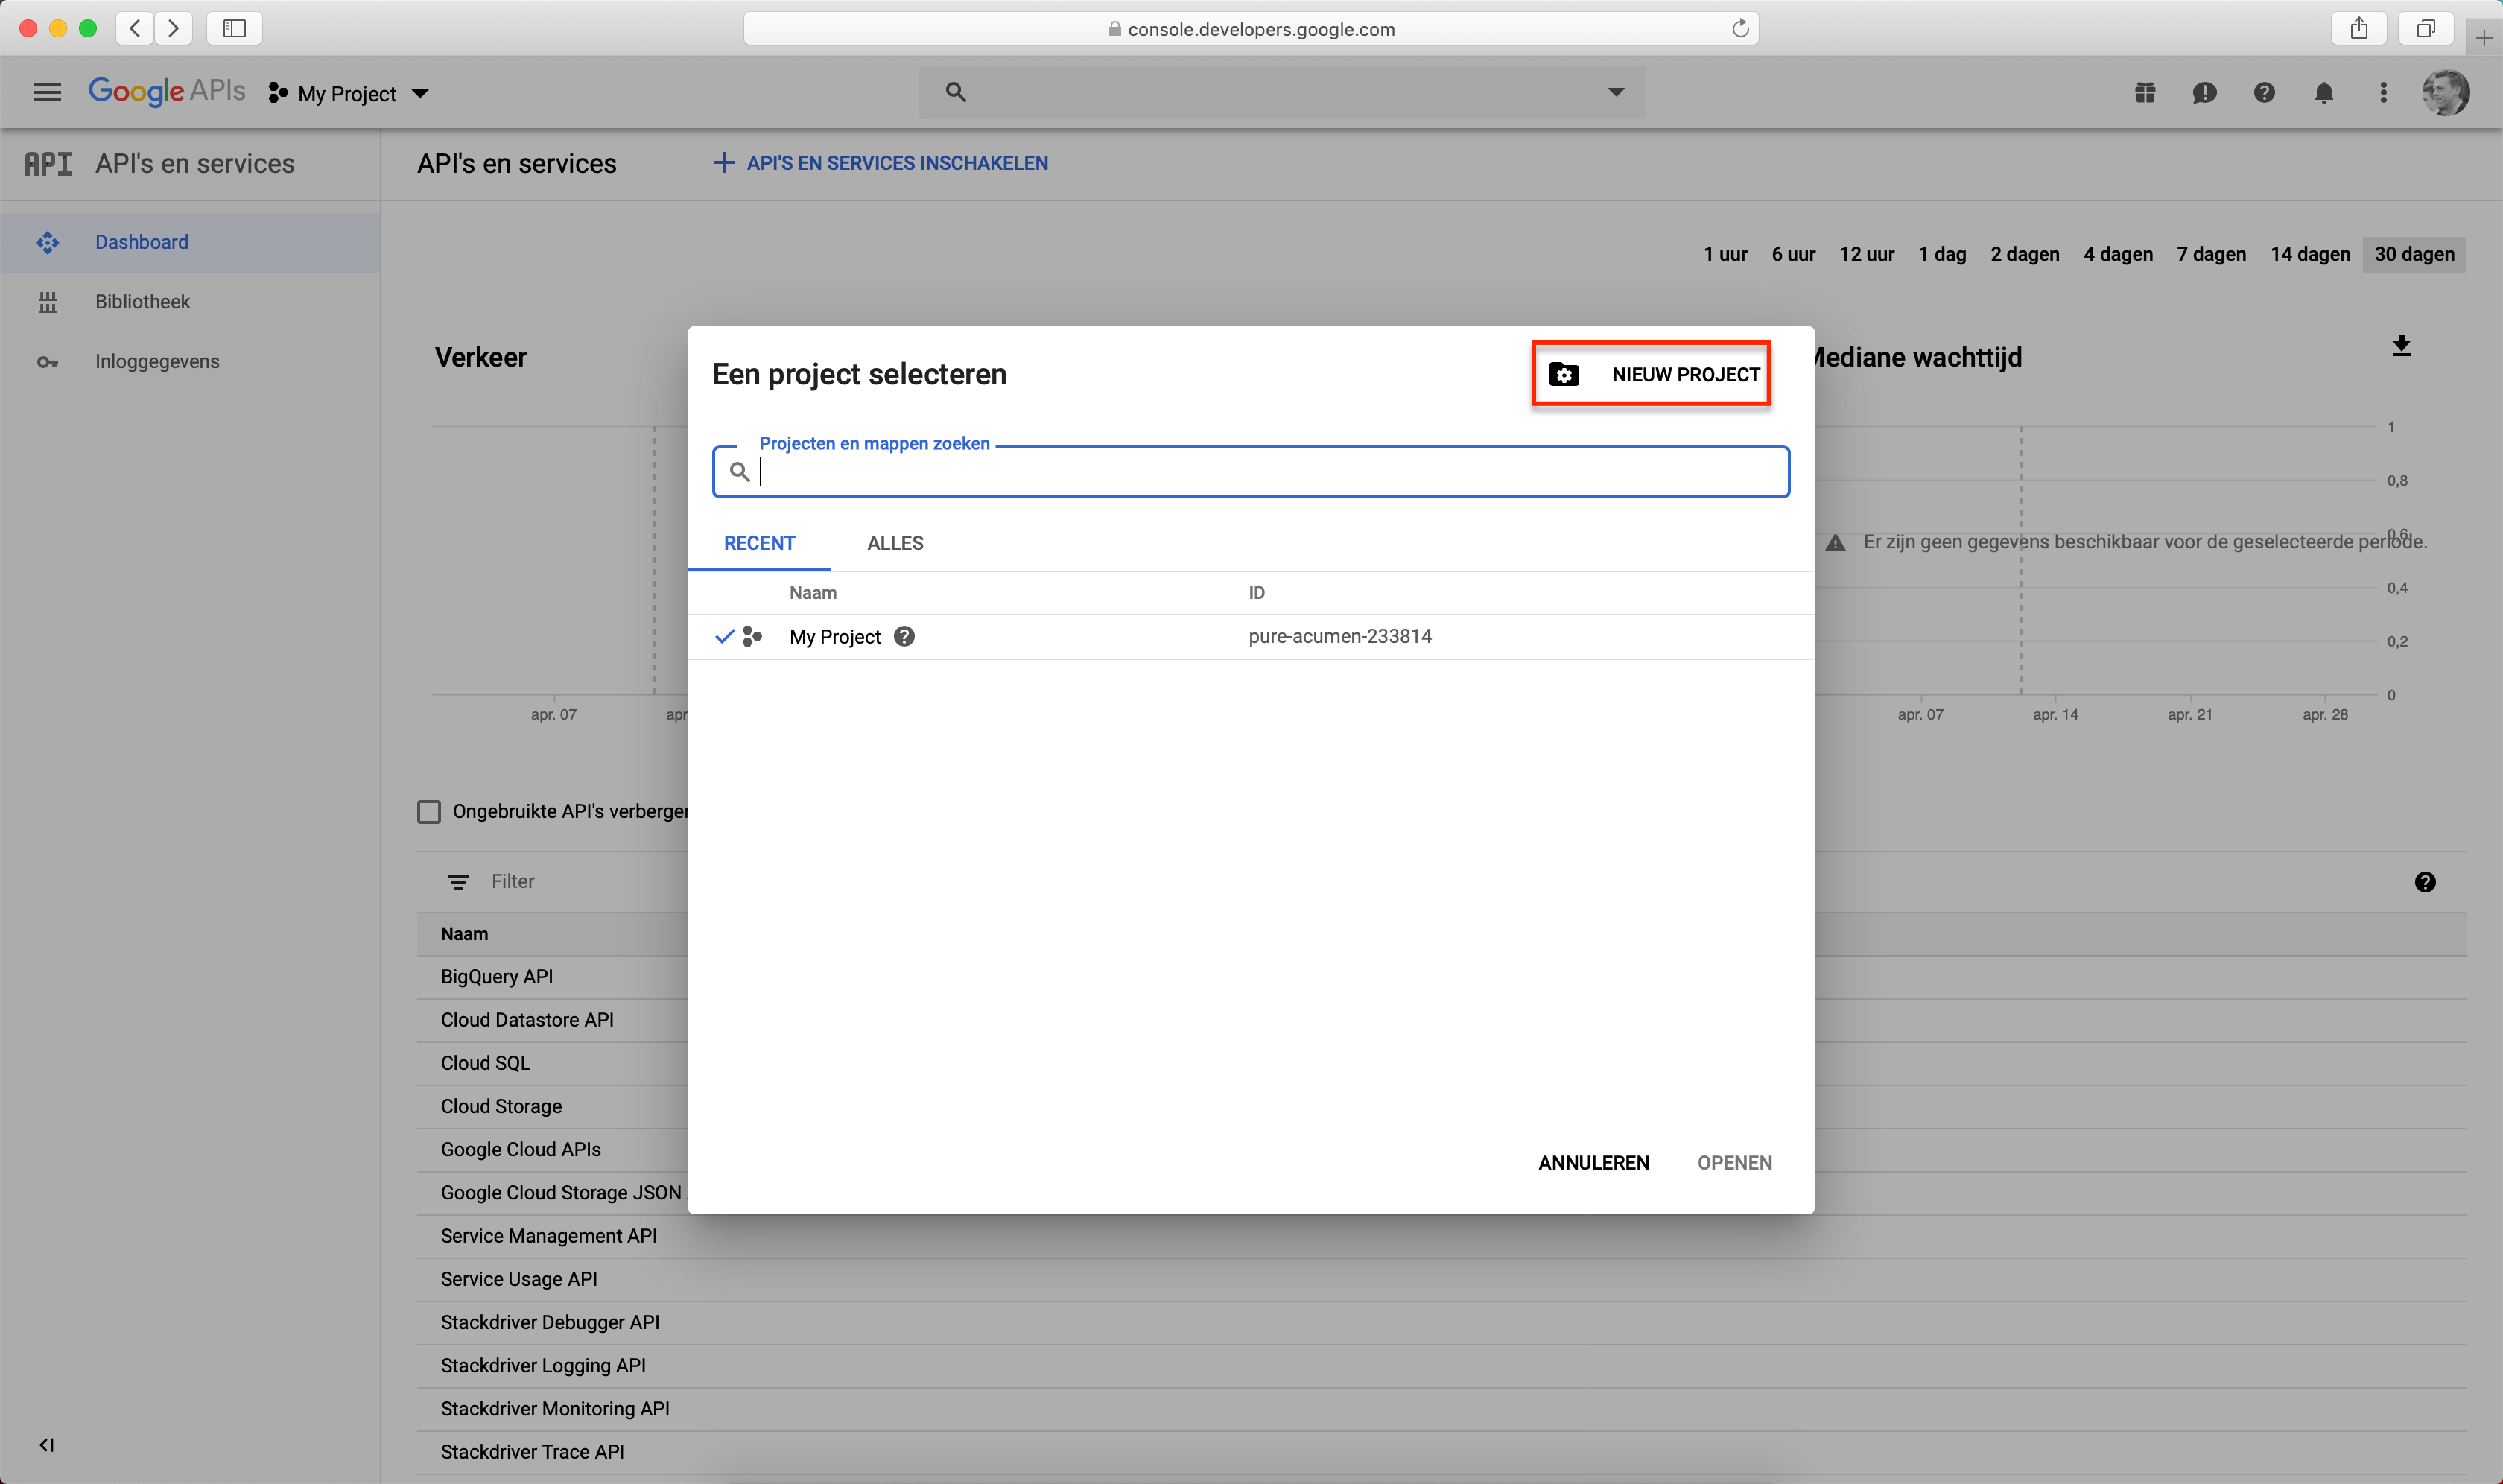
\includegraphics[width=0.9\linewidth,height=4.3cm]{img/google-sheets/gapi-maak-project.png}
        \captionsetup{width=0.8\linewidth}
        \centering
        \caption{Maak een nieuw Google Cloud project via de Google Cloud API console.}
    \end{subfigure}
    \begin{subfigure}{0.5\textwidth}
        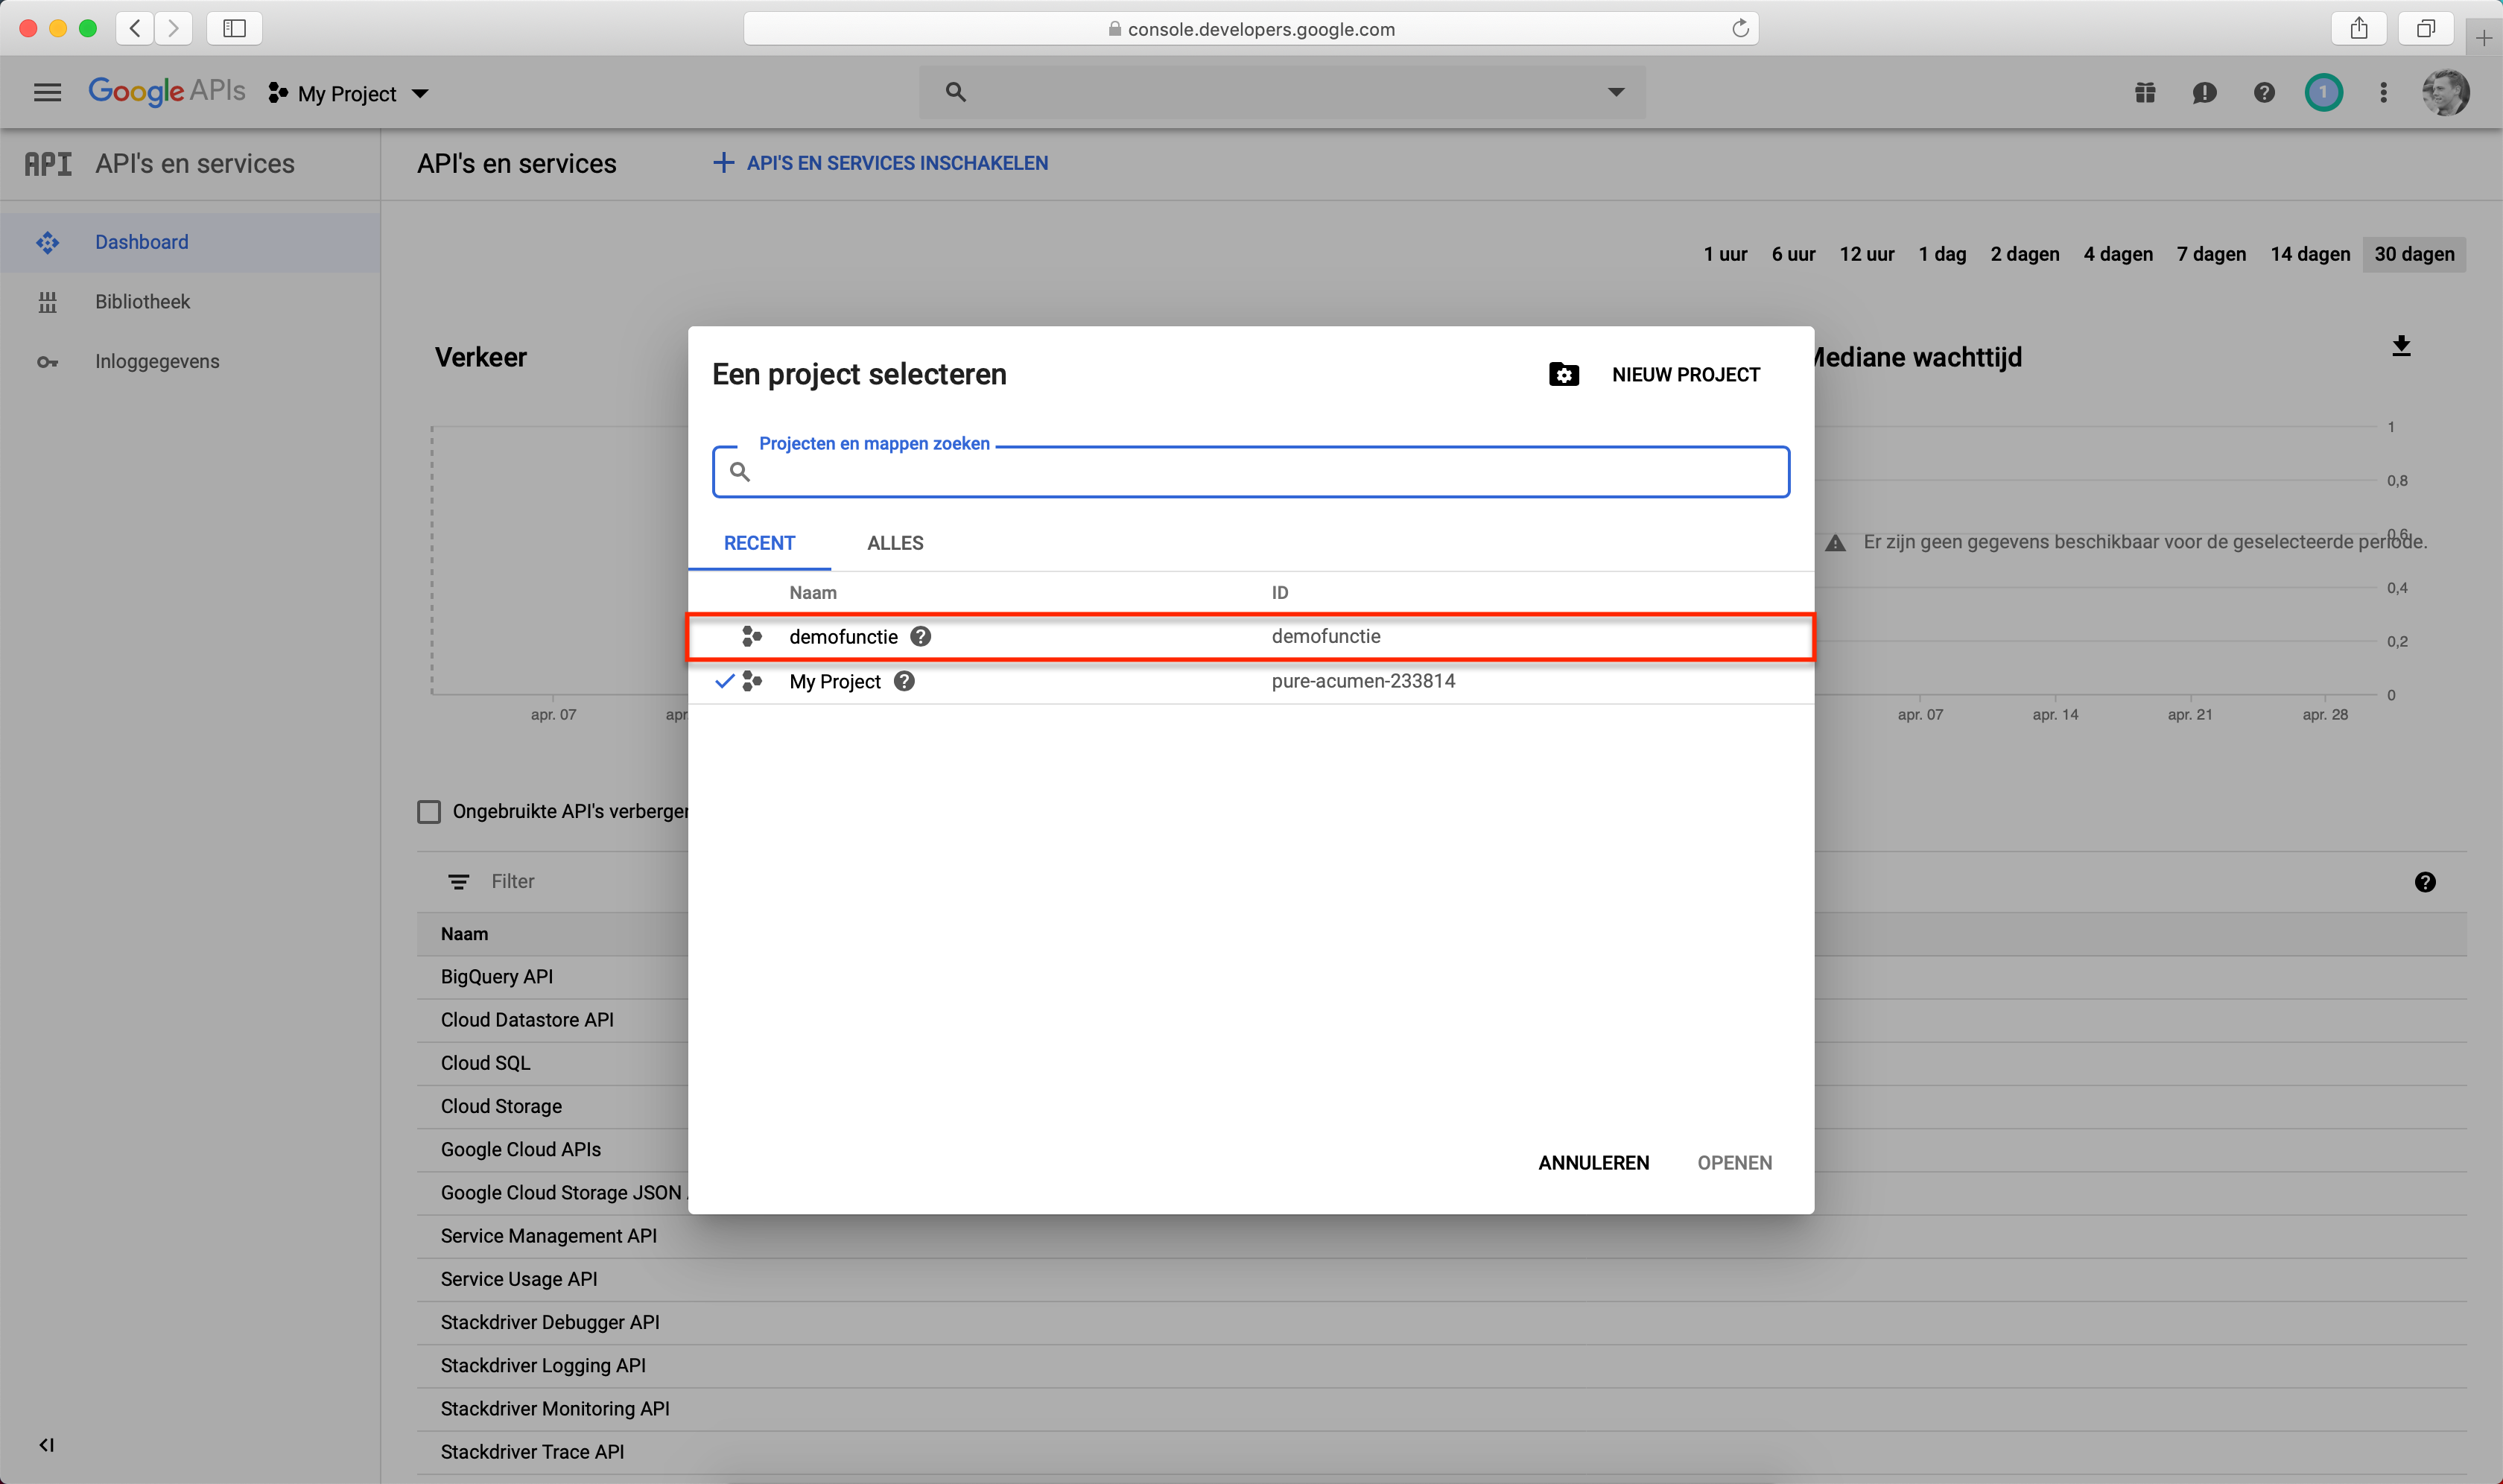
\includegraphics[width=0.9\linewidth,height=4.3cm]{img/google-sheets/gapi-selecteer-project.png} 
        \captionsetup{width=0.8\linewidth}
        \centering
        \caption{Selecteer het project dat zonet aangemaakt werd.}
    \end{subfigure}
\end{figure}
\begin{figure}[h]\ContinuedFloat
    \begin{subfigure}{0.5\textwidth}
        \captionsetup{width=0.8\linewidth}
        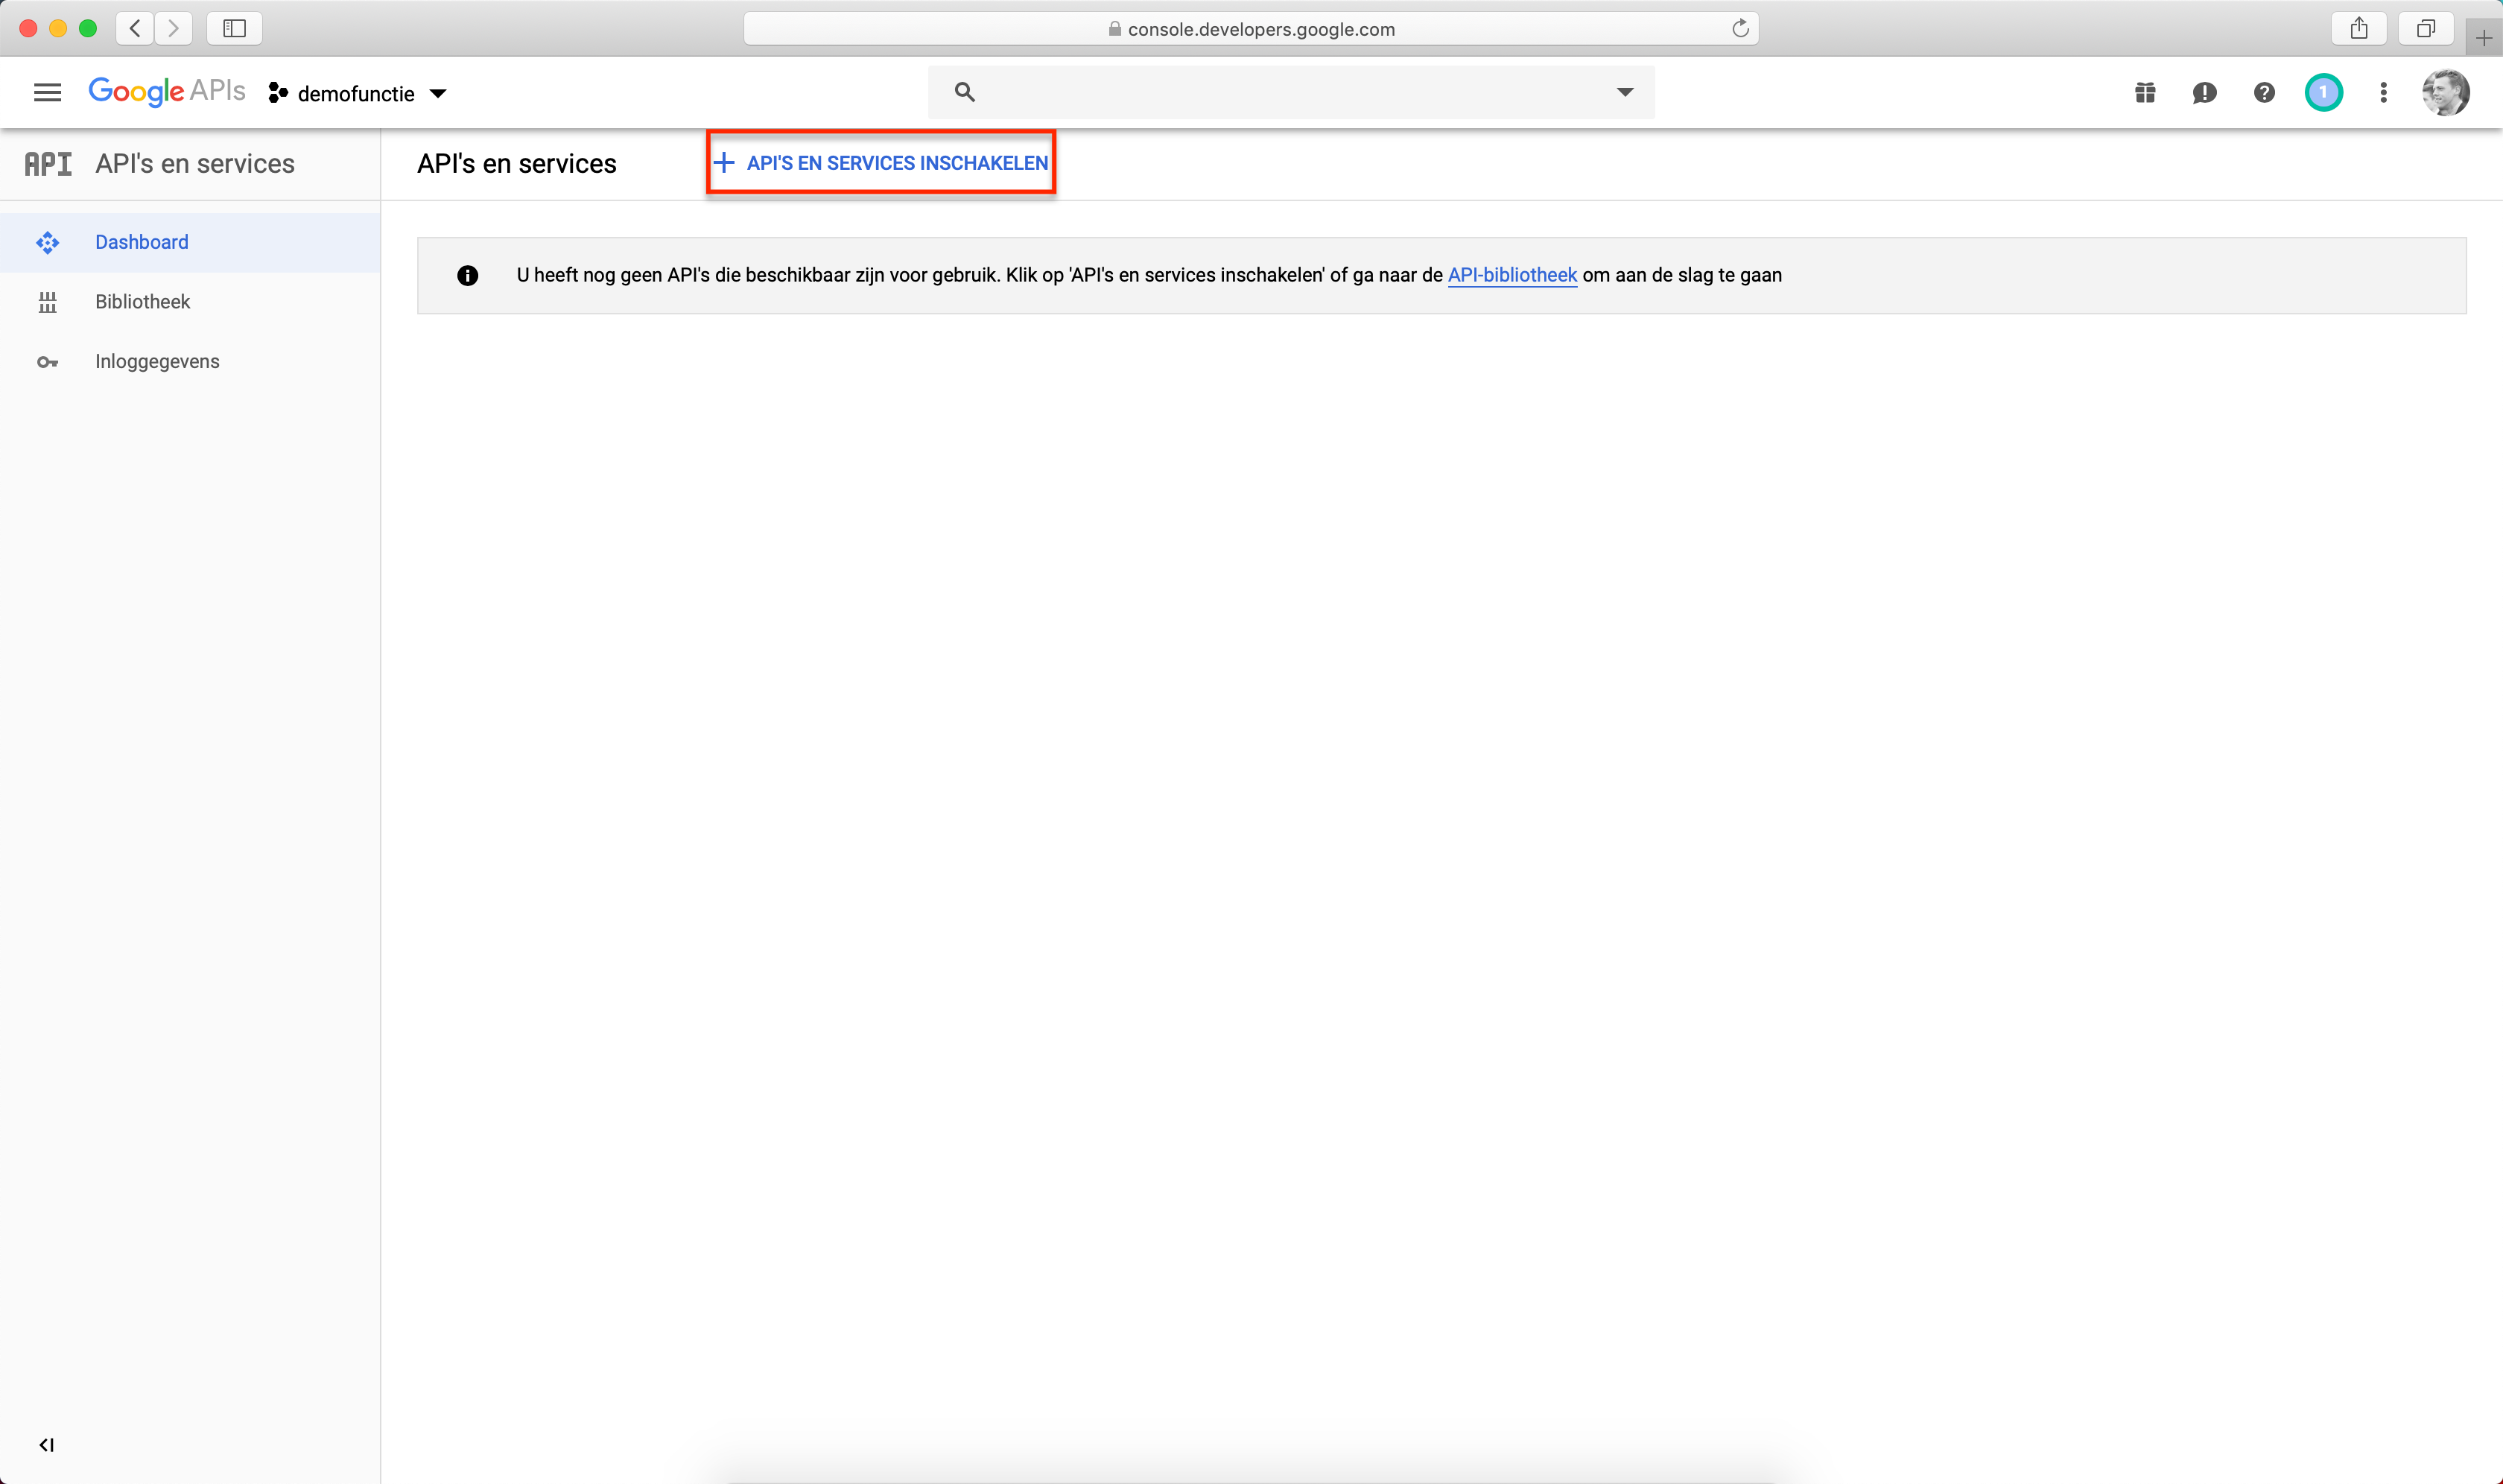
\includegraphics[width=0.9\linewidth,height=4.3cm]{img/google-sheets/gapi-api-inschakelen.png} 
        \centering
        \caption{Kies ervoor om API en services in te schakelen.}
    \end{subfigure}
    \begin{subfigure}{0.5\textwidth}
        \captionsetup{width=0.8\linewidth}
        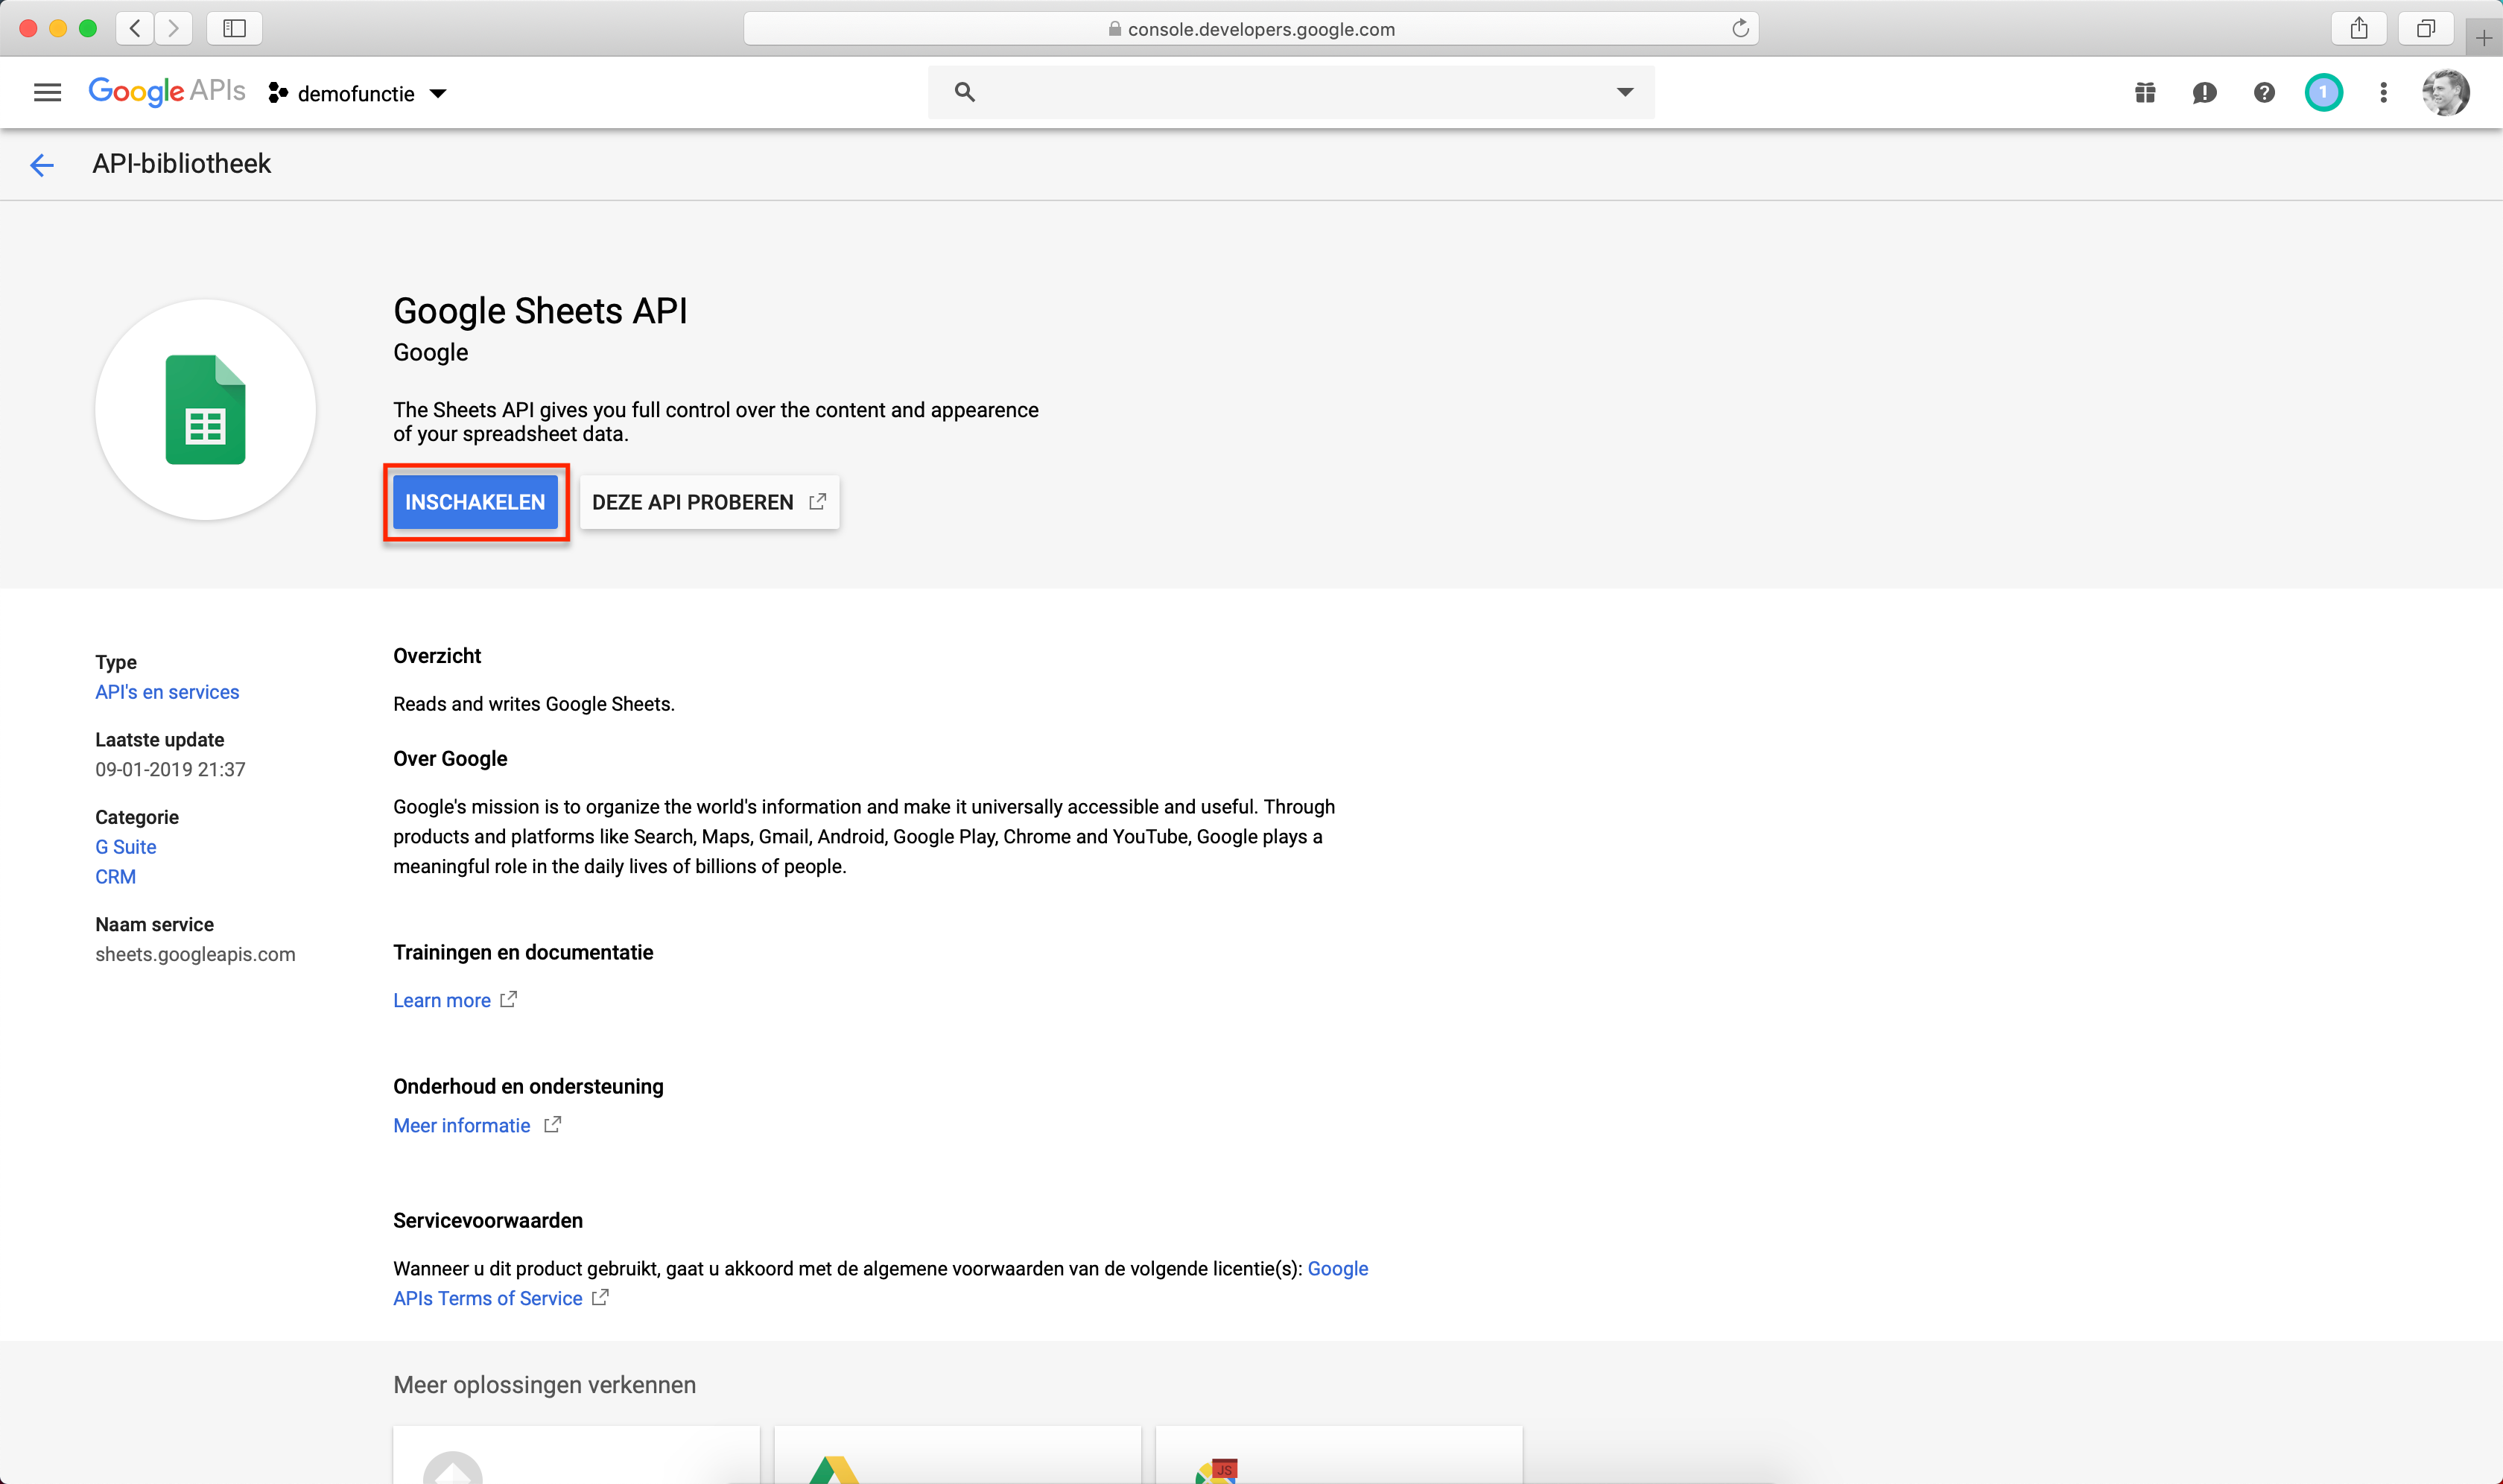
\includegraphics[width=0.9\linewidth,height=4.3cm]{img/google-sheets/gapi-google-sheets-api.png}
        \centering
        \caption{Zoek de Goolge sheets API en schakel deze in}
    \end{subfigure}
\end{figure}
\begin{figure}[h]\ContinuedFloat
    \begin{subfigure}{0.5\textwidth}
        \captionsetup{width=0.8\linewidth}
        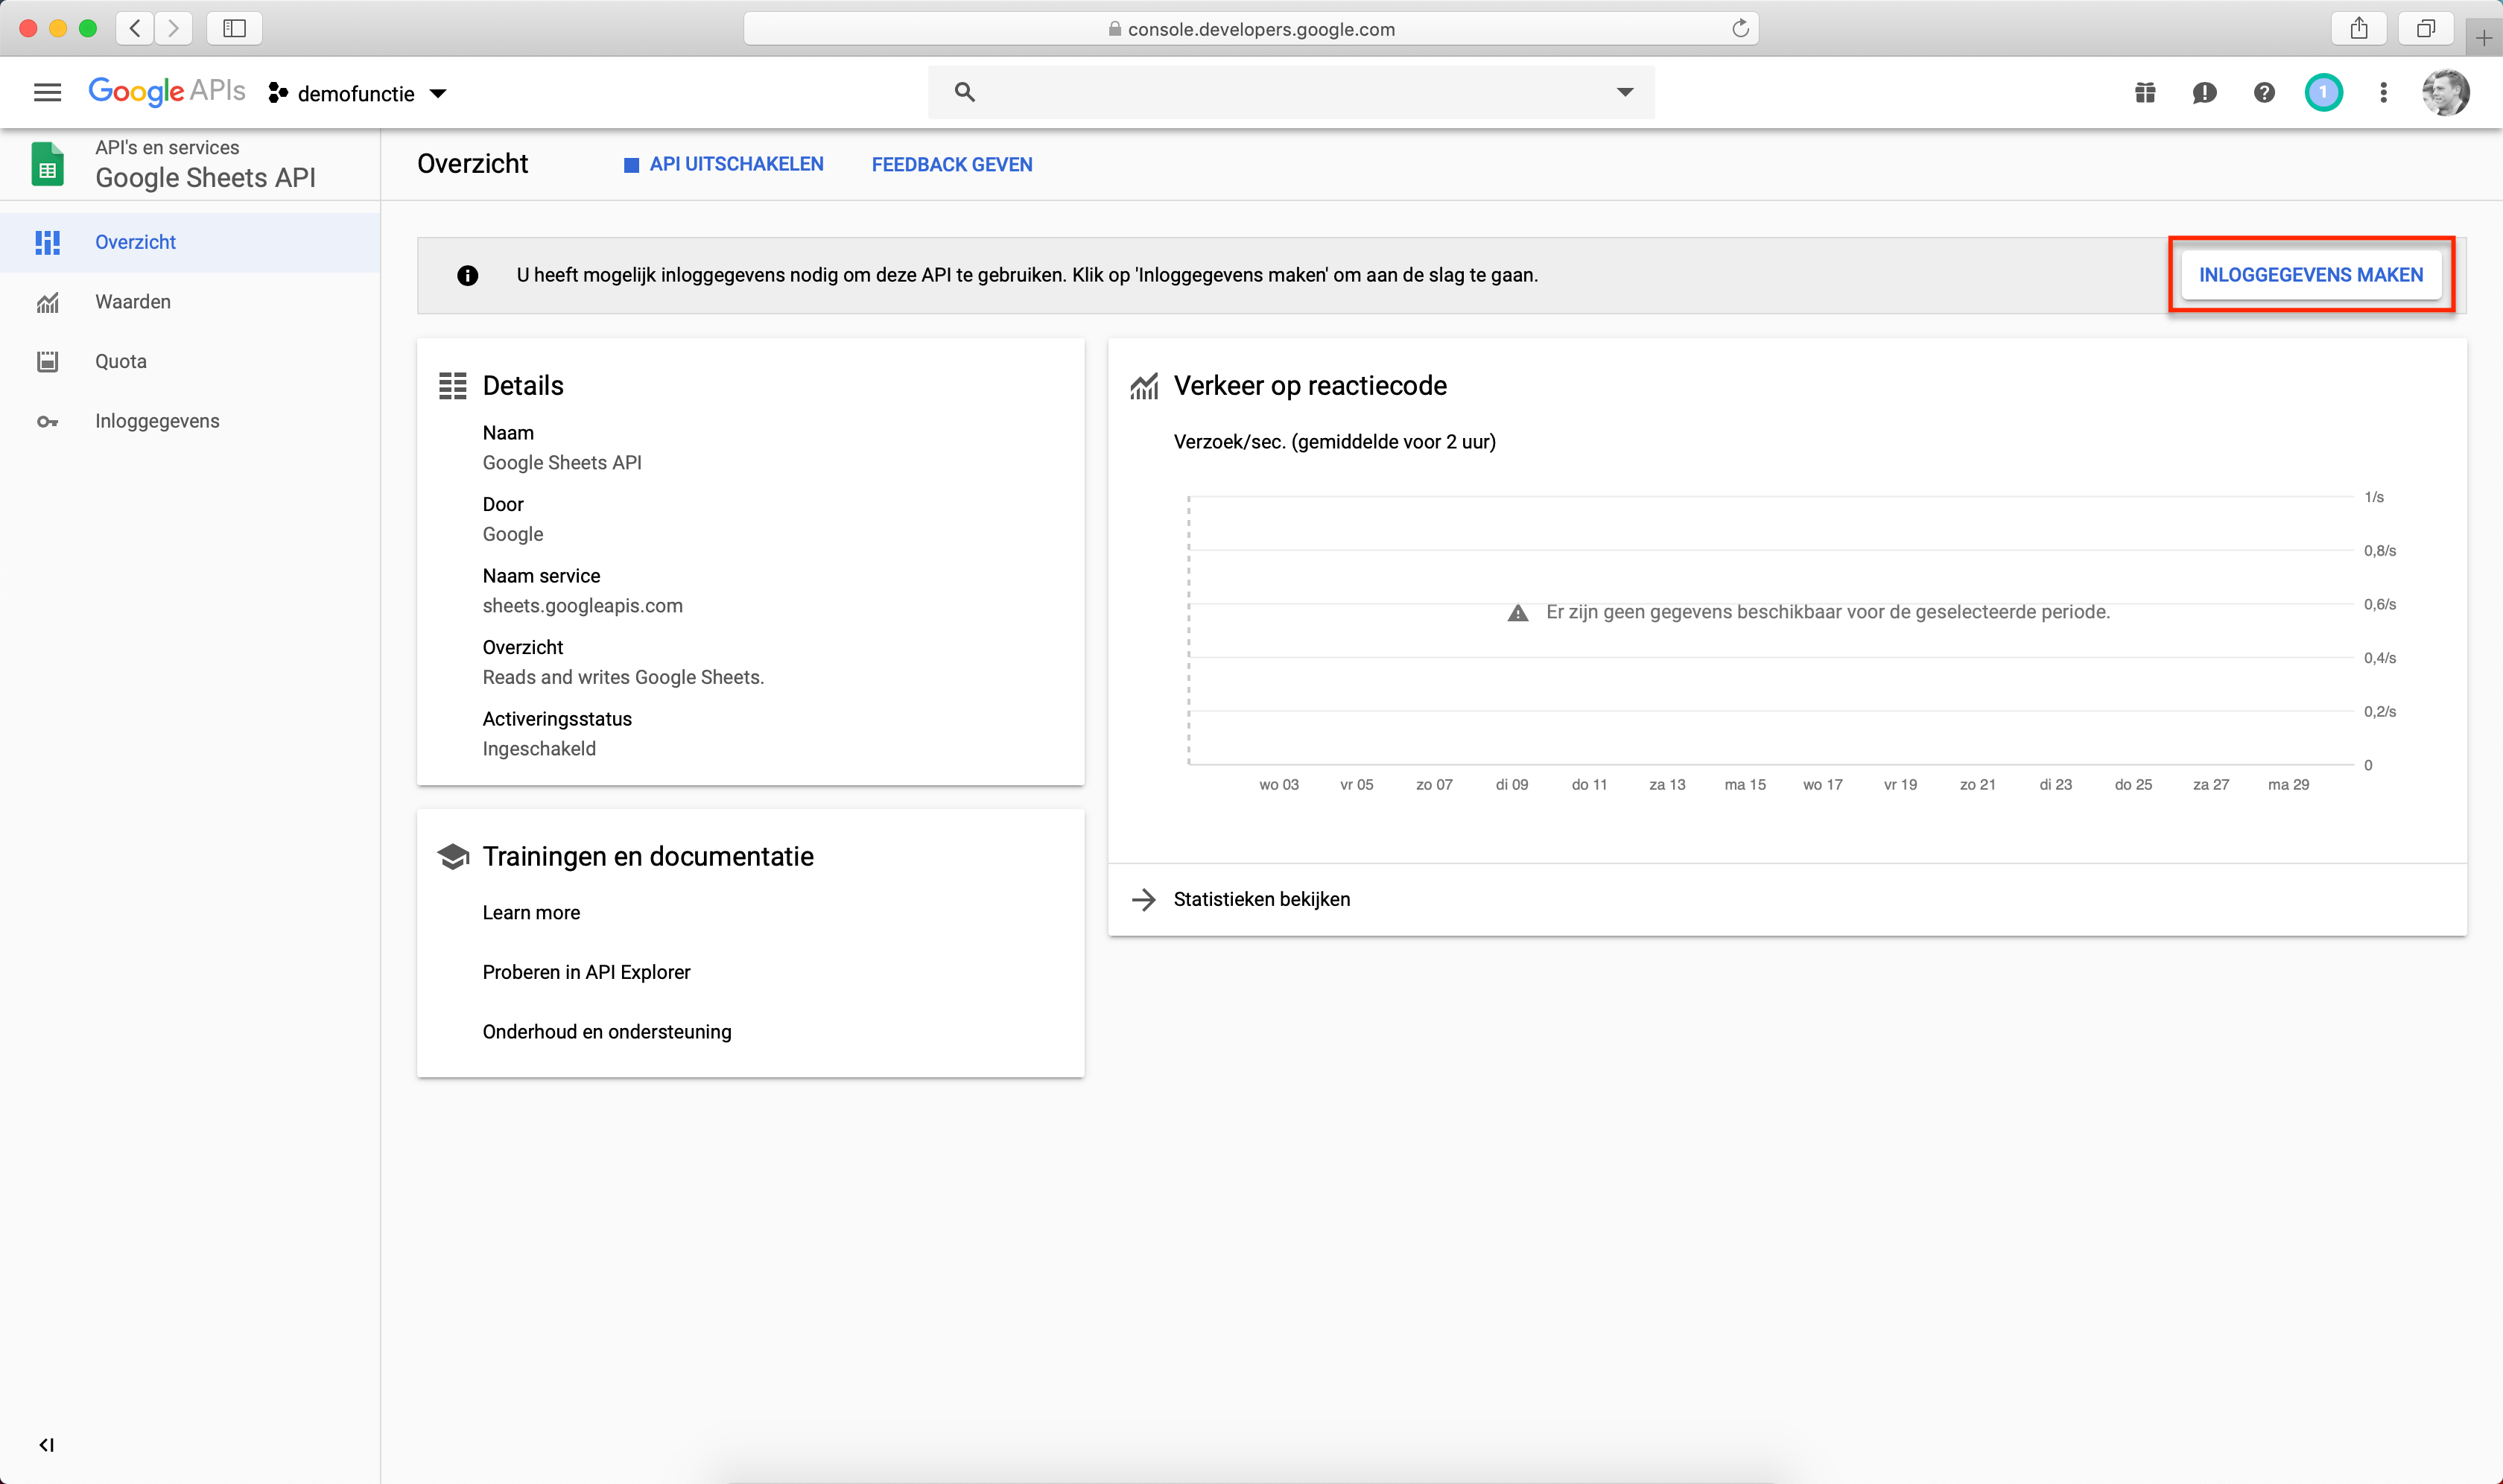
\includegraphics[width=0.9\linewidth,height=4.3cm]{img/google-sheets/gapi-maken-credentials.png}
        \centering
        \caption{Kies de optie om credentials aan te maken.}
    \end{subfigure}
    \begin{subfigure}{0.5\textwidth}
        \captionsetup{width=0.8\linewidth}
        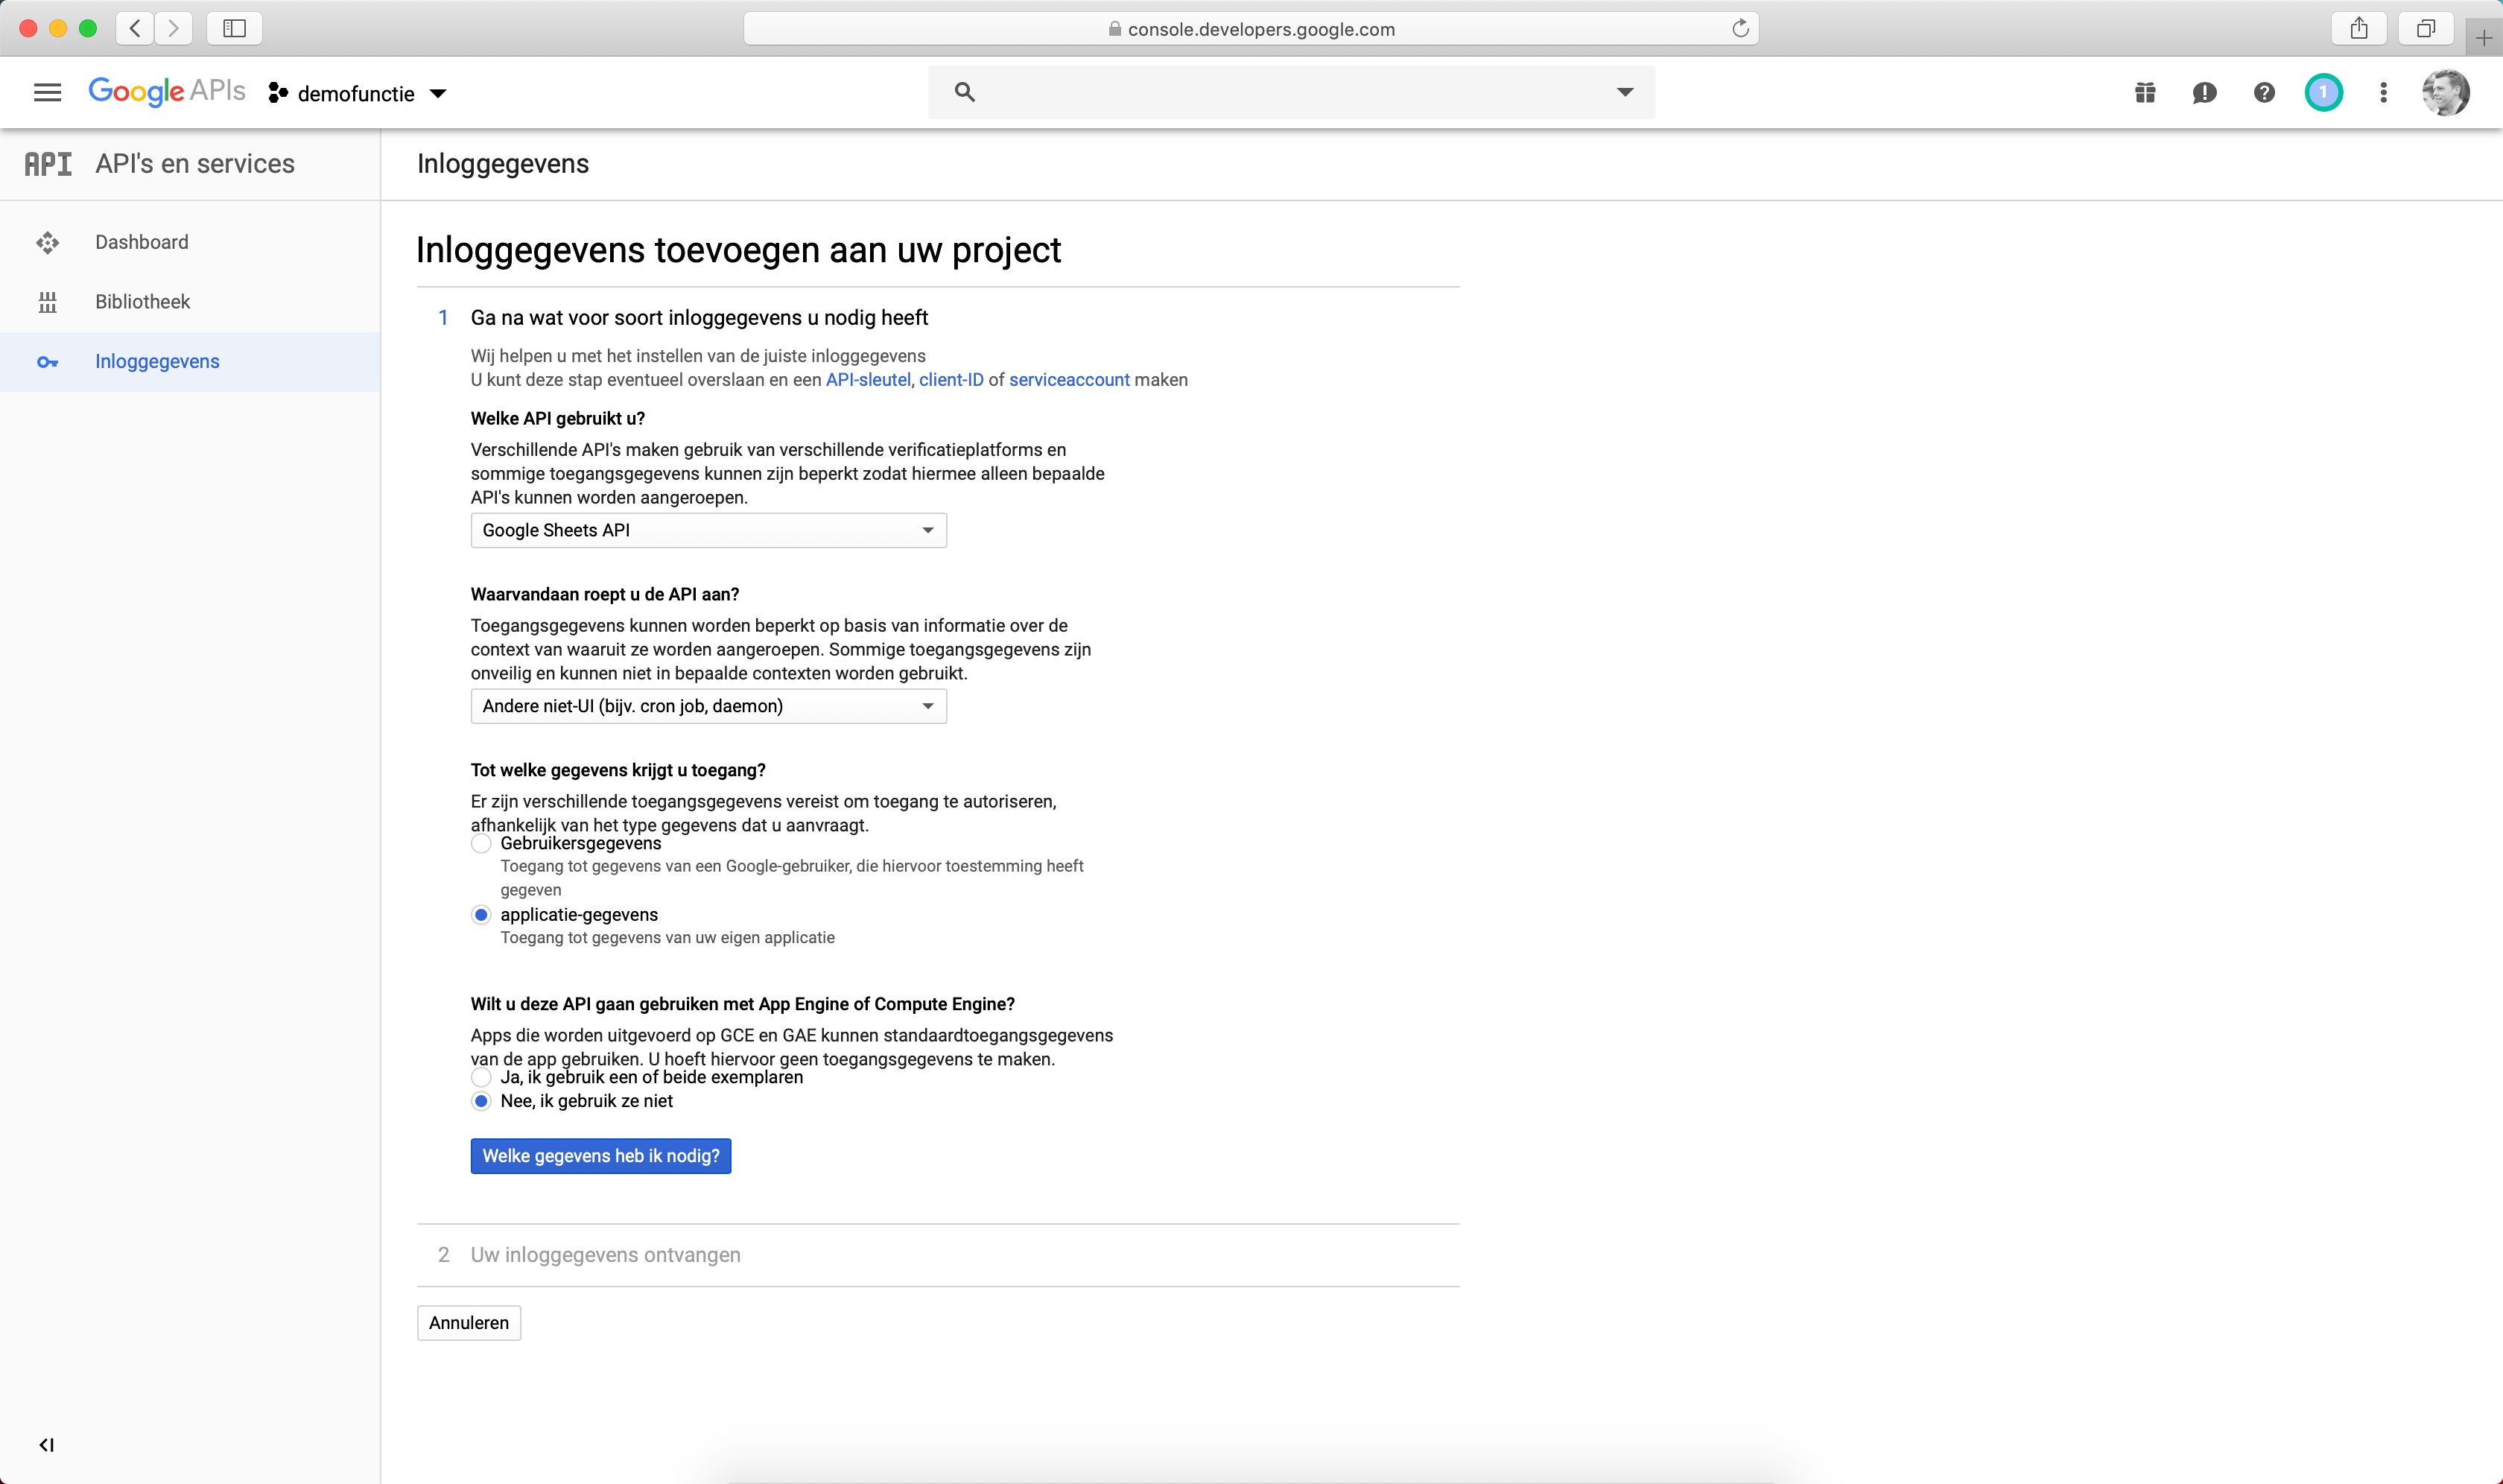
\includegraphics[width=0.9\linewidth,height=4.3cm]{img/google-sheets/gapi-credentials-1.png}
        \centering
        \caption{Invullen van gegevens voor credentials deel 1.}
    \end{subfigure}
\end{figure}
\begin{figure}[h]\ContinuedFloat
    \begin{subfigure}{0.5\textwidth}
        \captionsetup{width=0.8\linewidth}
        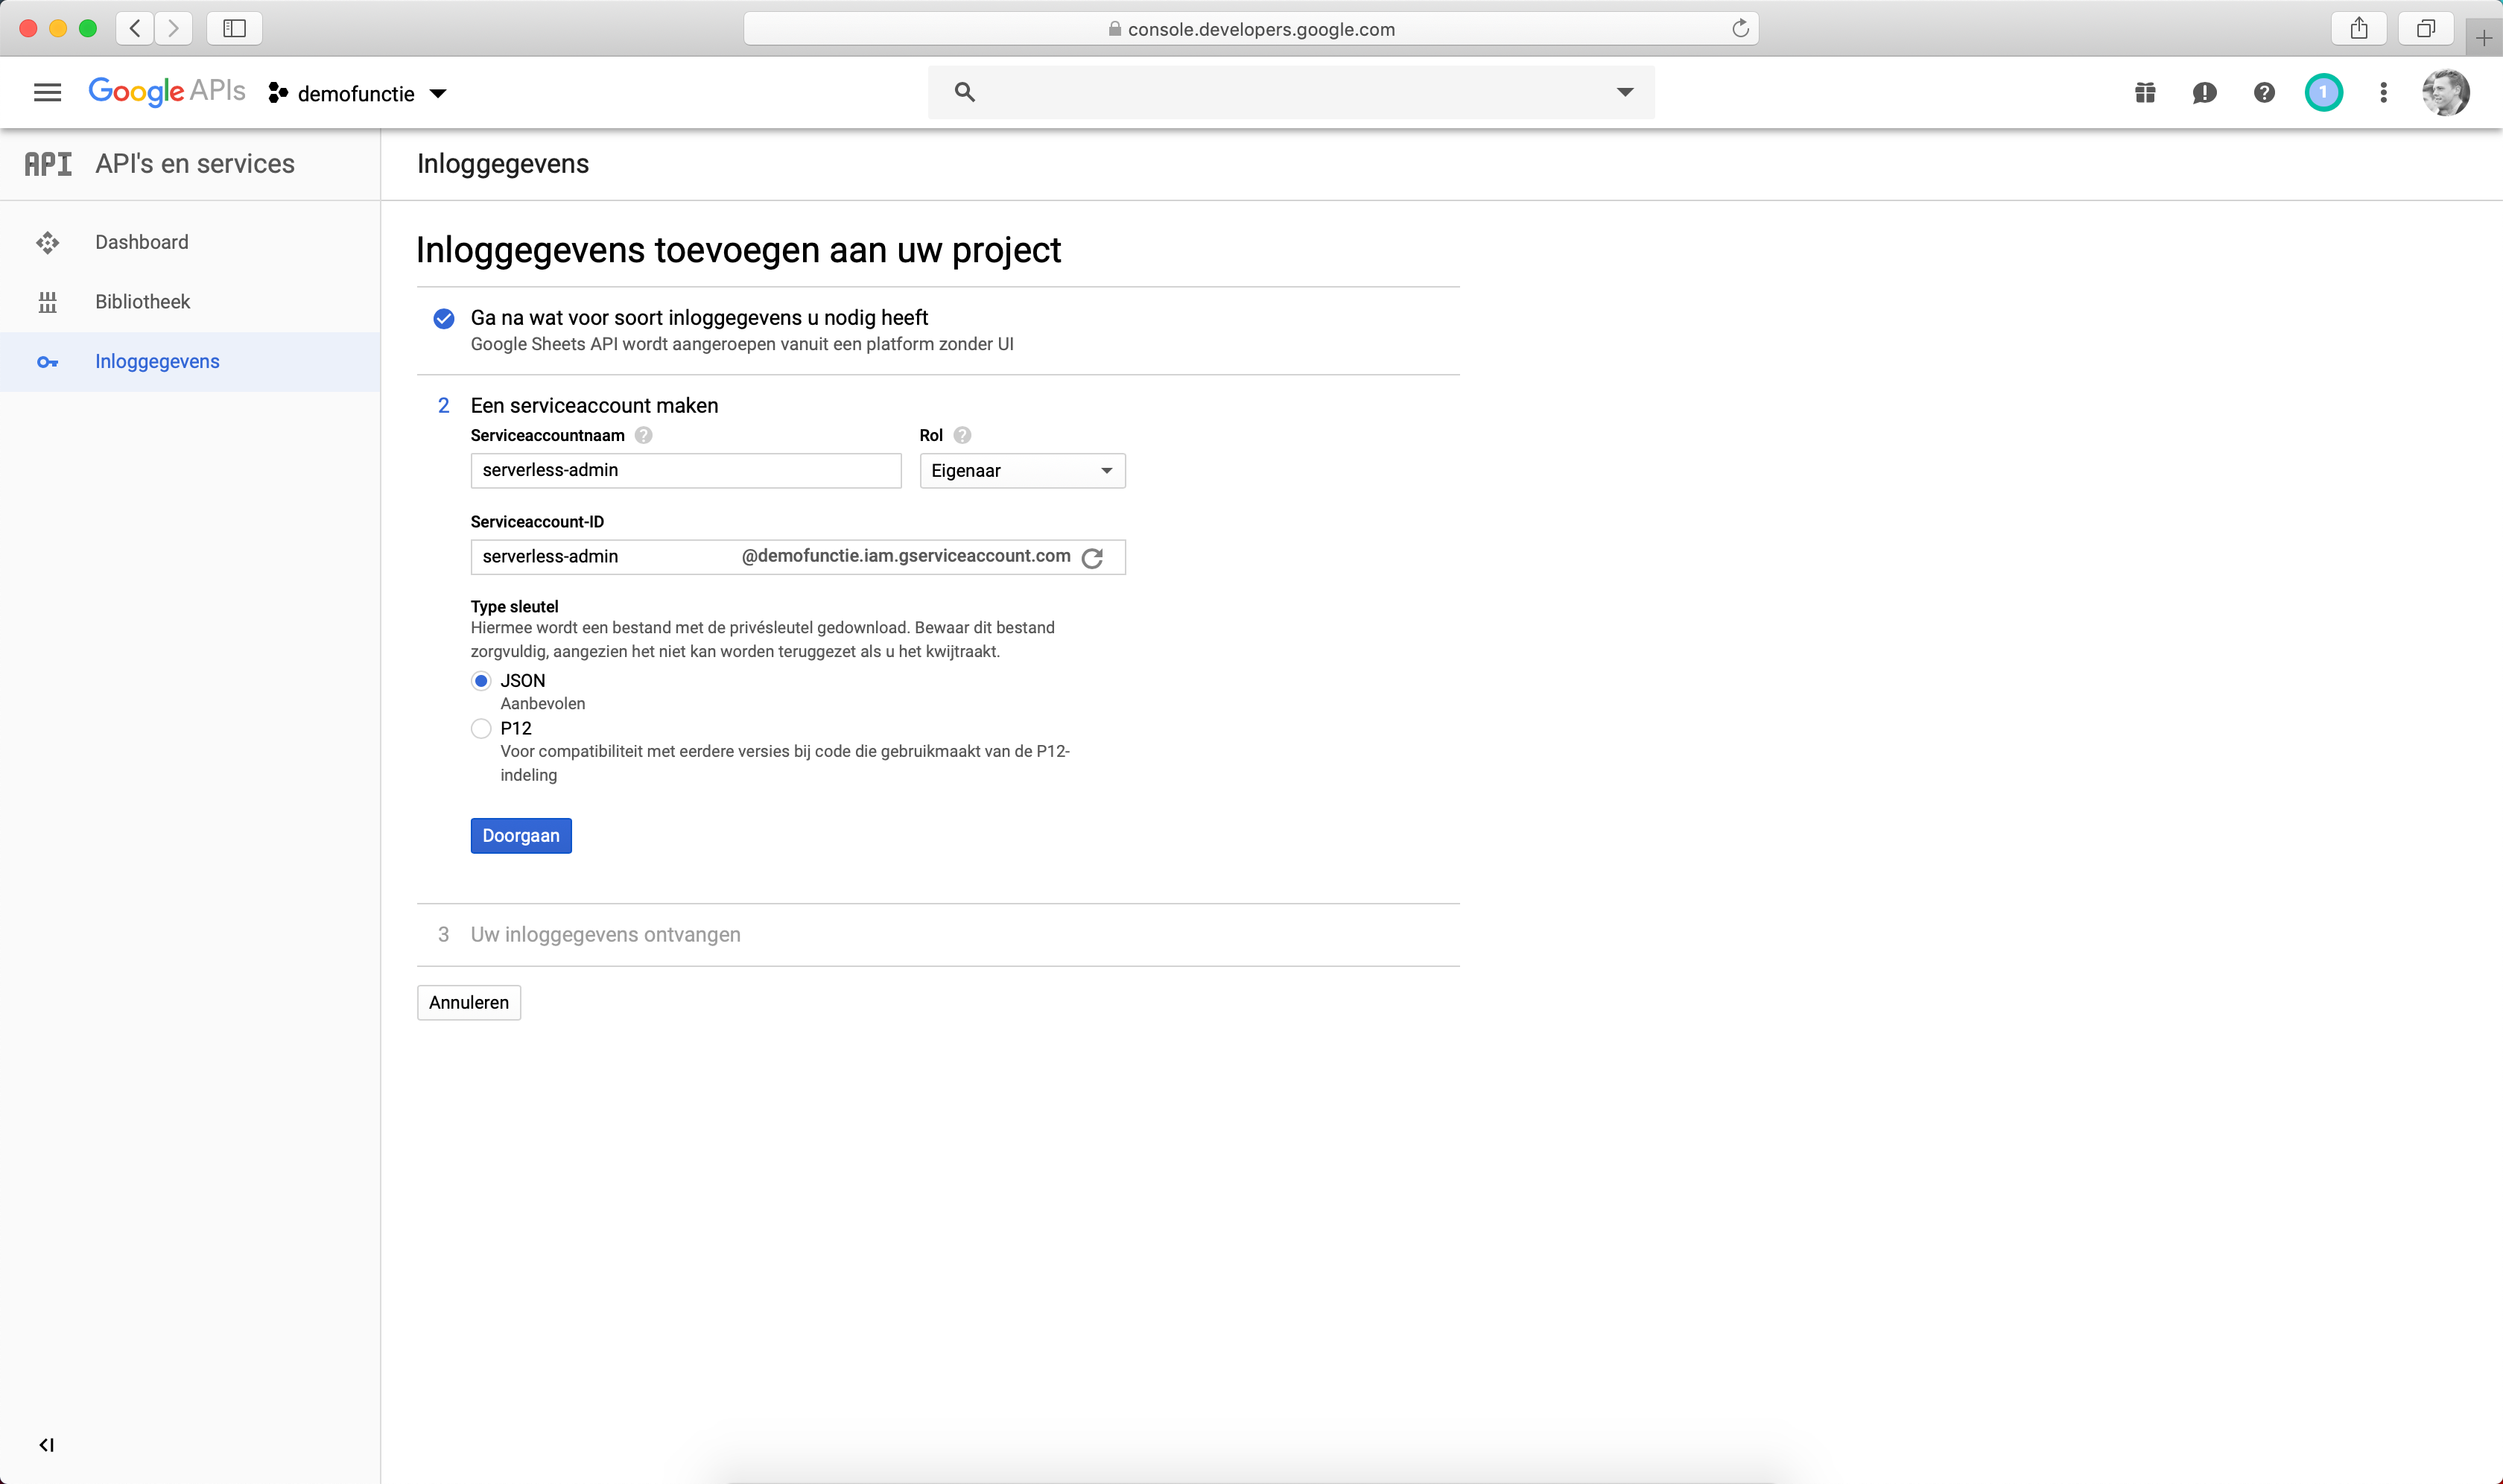
\includegraphics[width=0.9\linewidth,height=4.3cm]{img/google-sheets/gapi-credentials-2.png}
        \centering
        \caption{Invullen van gegevens voor credentials deel 2.}
    \end{subfigure}
    \begin{subfigure}{0.5\textwidth}
        \captionsetup{width=0.8\linewidth}
        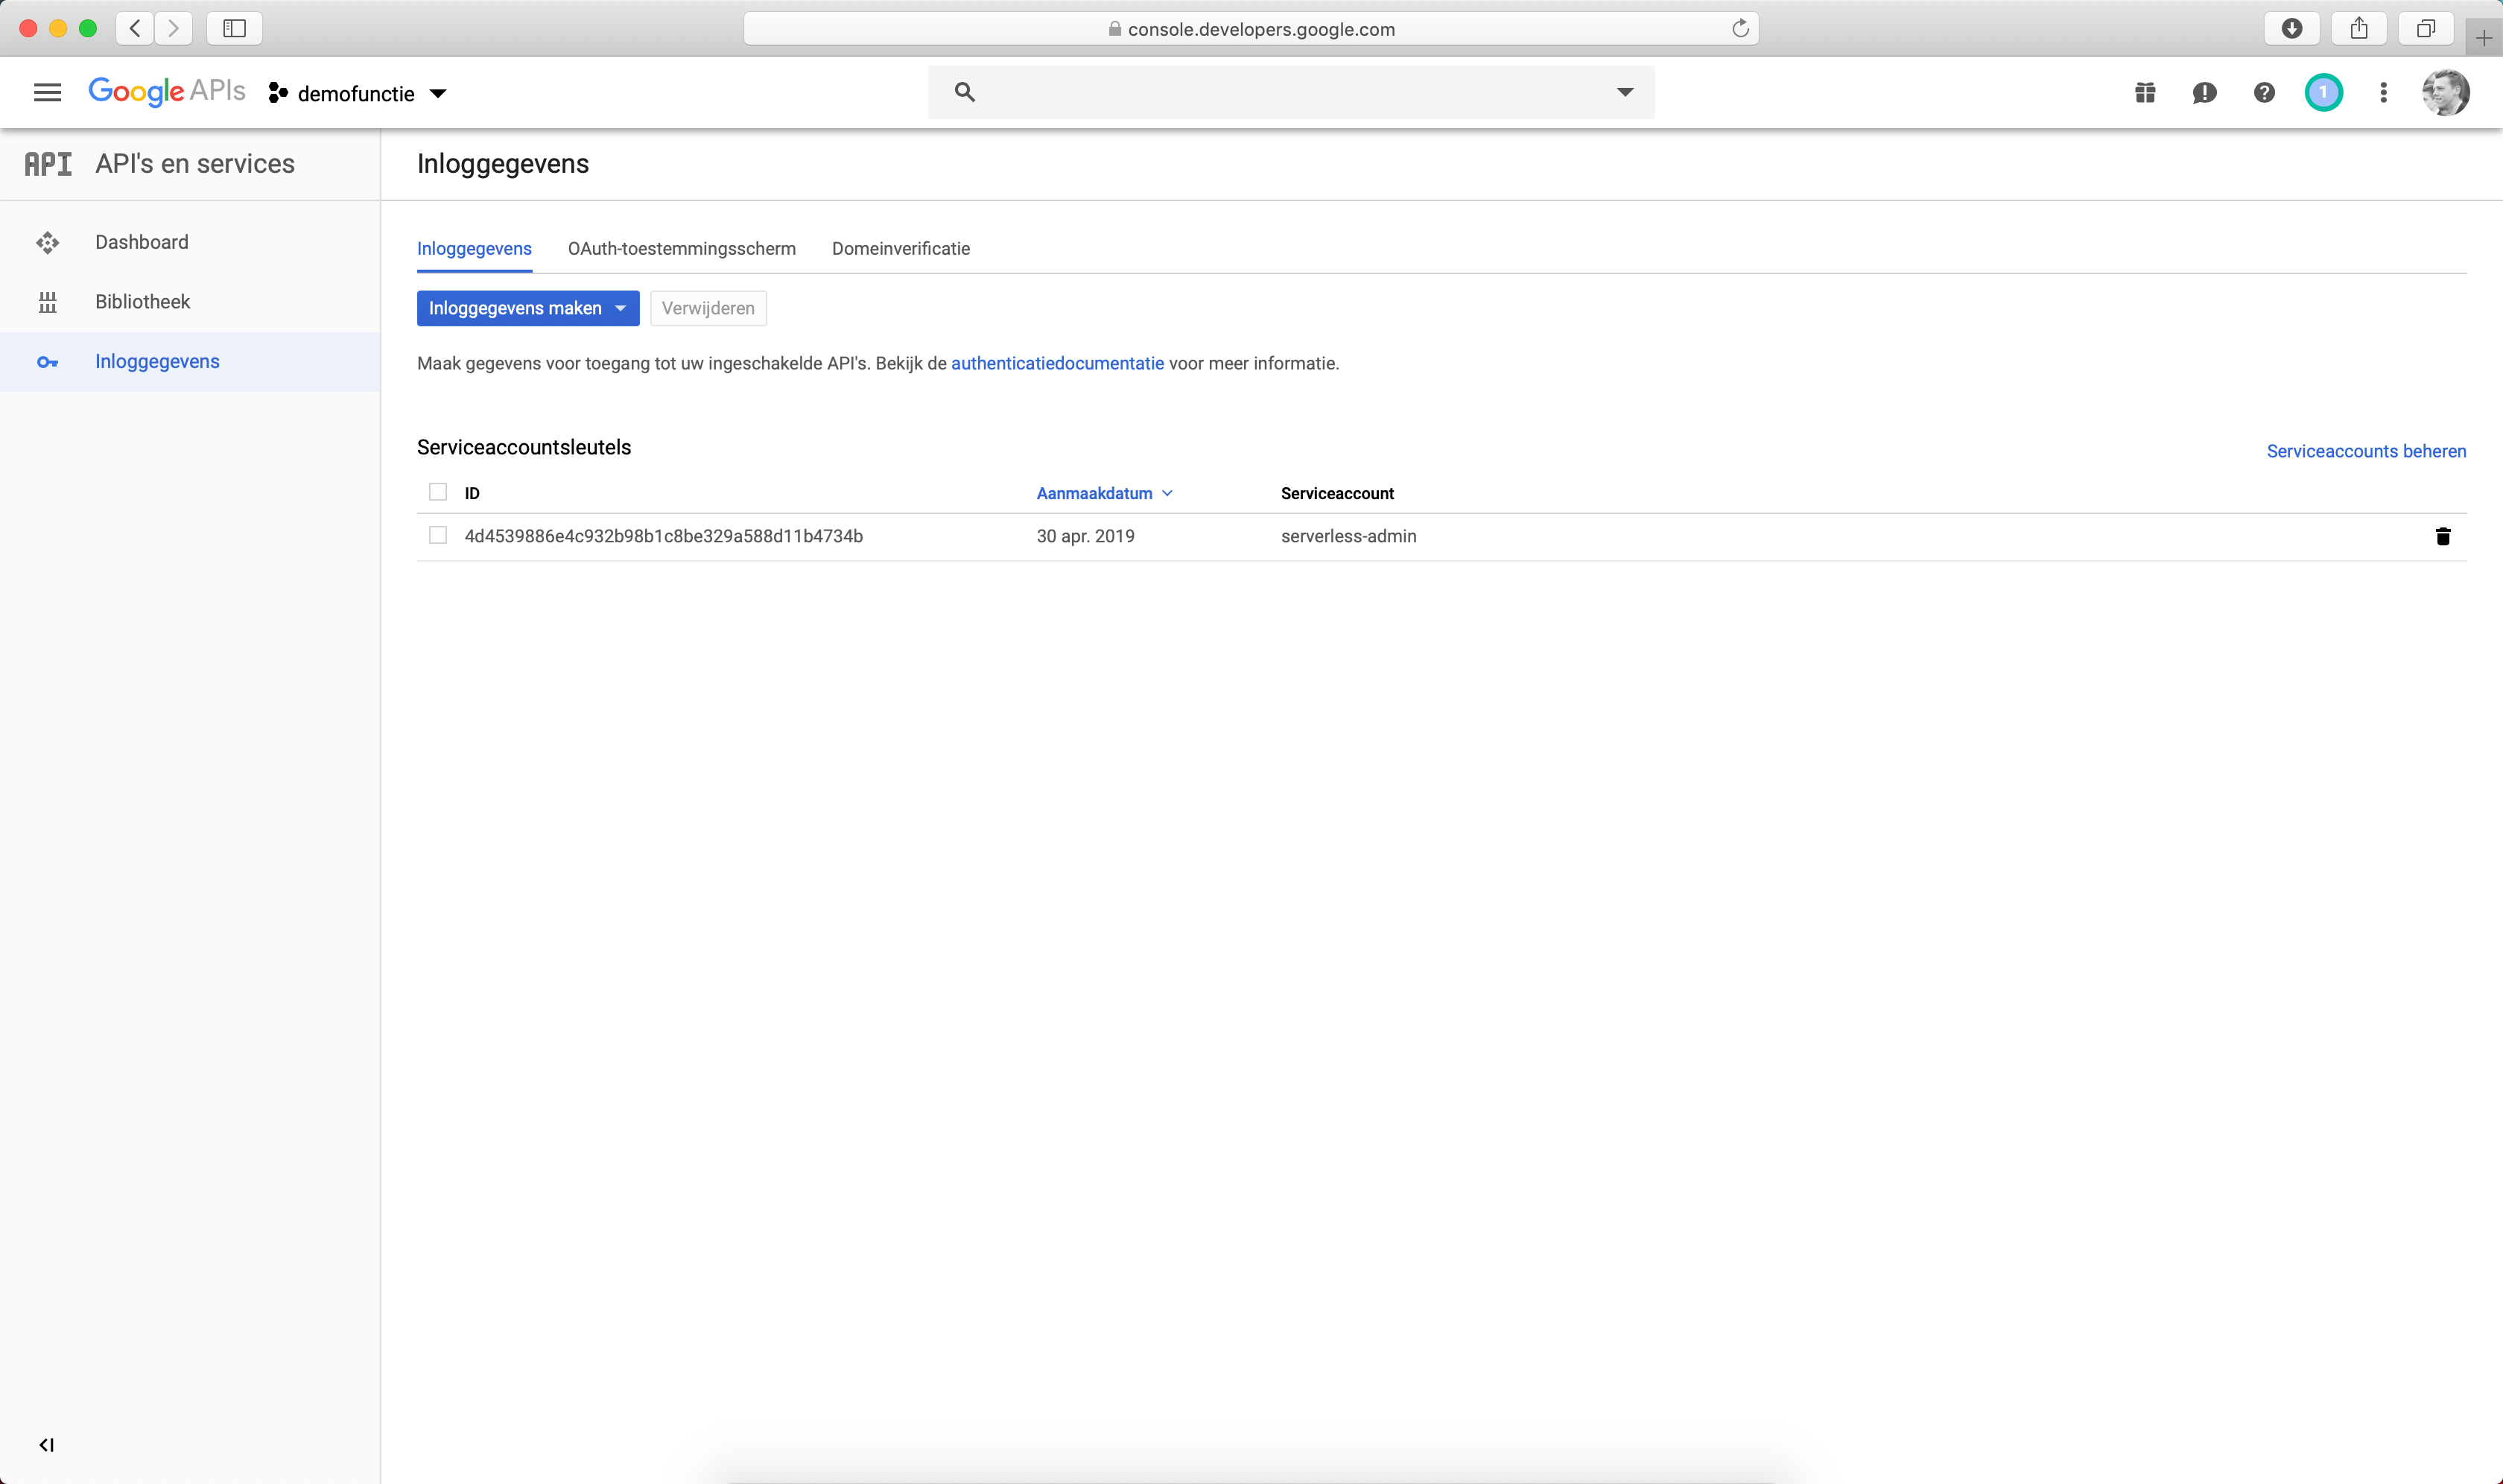
\includegraphics[width=0.9\linewidth,height=4.3cm]{img/google-sheets/gapi-credentials-3.png}
        \centering
        \caption{Credential account is nu beschikbaar.}
    \end{subfigure}
\end{figure}

Na het invullen van de gegevens voor het aanmaken van een credentials account wordt er automatisch een JSON bestand met de credential sleutel gedownload. Plaats dit bestand op een locatie waar het makkelijk is terug te vinden. Sla het bestand bijvoorbeeld op onder een map ''keys'' onder de home directory van de gebruiker.